\chapter{Background}

\section{Document management}

\subsection{General architecture of document management systems}

A document management system is a typical client-server model: a document
management server stores the documents in a document repository, which can be
accessed via various interfaces.  The other part of the system is a client,
which has built-in support for opening, saving and editing documents.

\begin{figure}[H]
\centering
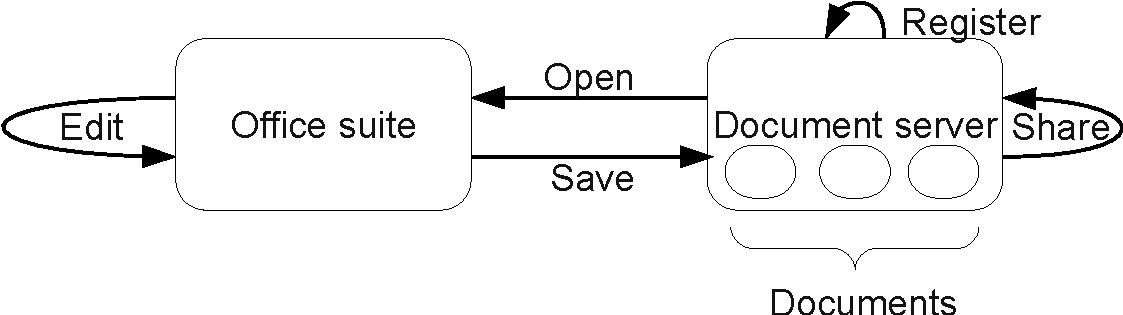
\includegraphics[width=450px,keepaspectratio]{general-arch-of-doc-mgmt-systems.pdf}
\caption{Architecture of a document management system}
\label{fig:general-arch-of-doc-mgmt-systems}
\end{figure}

\autoref{fig:general-arch-of-doc-mgmt-systems} shows the two entities of the
system. They have the following operations:

\begin{itemize}
\item The server primarily listens to client requests. Additionally it allows
performing operations directly on the server such as registering new users or
sharing documents of a user to others.
\item The client, connecting to one or more document server.
\end{itemize}

Every user can have access to document \textbf{workspaces}.\footnote{Users and workspaces are in an N:N relation: a user can have access to multiple workspaces and multiple users can use the same workspace.} Workspaces can have documents,
links and tasks. A workspace can be shared with different permissions
(read-only, read-write), and that is typically done by sending an invitation
email which can be accepted by the other user.

A user may access the document server using a web browser, or via rich client
applications. The advantage of the web browser interface is that it can be
accessed from almost everywhere, however, document editing can't be performed.
If such operation should be performed, then the user has to manually download
the document, edit then upload it. This method occasionally does not cause a
problem, but of course it is uncomfortable for daily work.

The other interface is a rich client, which is installed on the machine of the
user. Vendors prefer to produce a corresponding client for their server,
Microsoft SharePoint and Microsoft Office is a typical setup.

In case of servers or clients speaking different communication protocols,
selection of the used protocol is selected differently on client and server
side. Servers can listen on different addresses, and in this case the address
identifies not only the server, but the used protocol as well.

For example Alfresco, has its native protocol, but also (more or less) provides
support for the SharePoint protocol. As a result, it can be configured to
listen on one URL as an Alfresco server, and on an other URL as a SharePoint
server. Additionally, it even supports CIFS, FTP and NFS for some
operations. \cite{alfresco-fsc}

Clients can have different extensions or plug-ins to handle different
protocols. For example Microsoft Office can accept SharePoint URL-s in the
standard file opener dialog, while the Alfresco extension for OpenOffice.org
has a dedicated menu in the application to connect to an Alfresco server.

It is also common that the client extensions have minimal business logic. For
example the proprietary SharePoint extension to OpenOffice.org, created by
Oracle can't talk to every SharePoint server, but Microsoft Office does -- as
long as a server-side component provided by Oracle is not installed on the
server. While this approach may be compelling during development, actually it
is uncomfortable for system administrators.

\subsection{Related standards}

\begin{figure}[H]
\centering
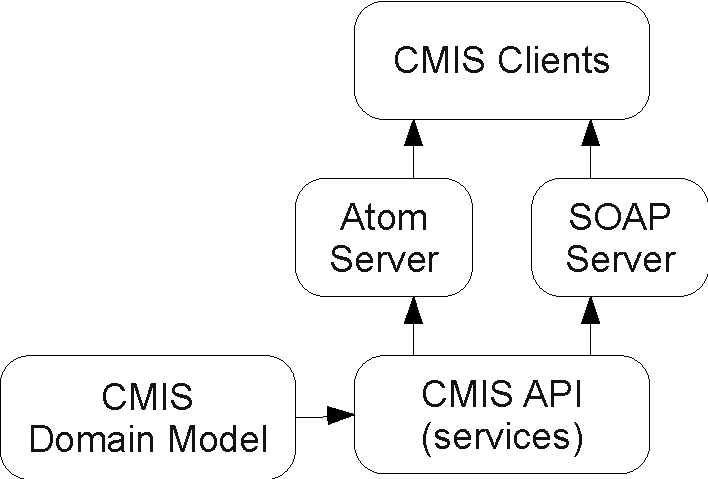
\includegraphics[width=250px,keepaspectratio]{cmis.pdf}
\caption{Architecture of the CMIS standard}
\label{fig:cmis}
\end{figure}

The specification called Content Management Interoperability
Services \cite{cmis} is created to address compatibility issues between various
document management server implementations. OASIS approved it on May 1, 2010.
Also, at the time of writing implementation is far from complete among major
document management servers. Alfresco 3.3+ implements the client side only,
SharePoint 2007 does not support it yet, so at the moment it is a vision that
all major document servers will implement this specification.

On the other hand, there are a lot of implementations in other products, such
as IBM Lotus Connections 3.0 \cite{lotus} (server side only) or TYPO3 (client
and server side).

CMIS has two main goals:

\begin{itemize}
\item Providing a list of web service (SOAP) interfaces, it is language-independent.
\item It allows separating the service and content, making it possible to
implement services for legacy document repositories without modifying them.
\end{itemize}

To achieve this, it defines a domain model, describing the following data model
elements (see \autoref{fig:cmis}):

\begin{itemize}
\item repository: A container for objects.
\item object: Common ancestor for document, folder, relationship and policy objects.
\item object-type: A set of properties, all instances of a type have those.
\item document object: The document entities managed by the repository.
\item folder object: Container for file objects.
\item relationship object: Representing links between objects.
\item policy object: Policies enforced by a repository.
\item access control: Consists of pre-defined permissions and allows defining new ones.
\item versioning: Versions document objects (other object types are not allowed).
\item query: Type-based query to list objects matching a specified criteria.
\item change log: Changes to objects since a given timestamp.
\end{itemize}

Then -- using this data model -- it specifies services to operate on them:

\begin{itemize}
\item common service elements: Includes paging, exception handling.
\item repository services
\item navigation services
\item object services: Includes factory functions for different object types.
\item multi-filing services: Makes it possible to add/remove objects to folders.
\item discovering services: To search query-able objects within a repository.
\item versioning services: Includes check in, check out, cancel checkout, get
	versions.
\item relationship services: Provides the relationships of an object.
\item policy services: Apply and remove policies, list applied ones.
\item ACL services: Get and apply an ACL.
\end{itemize}

Finally it explains concrete syntaxes: the Restful AtomPub Binding and the Web
Services (SOAP) binding.

\subsection{Concrete implementations}

In this subsection, we give a short comparision of Microsoft SharePoint 2007 and
Alfresco Community Edition 3.4, which claims to be "The Open Source Alternative
for Enterprise Content Management".

A general notable difference is that Alfresco does not allow deletion where
possible. Of course it is possible to delete documents, but it isn't possible
to delete document versions, overwrite a previous document version or delete a
whole workspace as a single operation.

On the other hand, SharePoint uses its leading position to avoid publishing
proper documentation on how communication protocol it uses works. This protocol
existed before the CMIS standard was published, and it is not a standard. For
example the \emph{put document} method has a \emph{document} parameter -- the
documentation \cite{spdoc} does not mention the \emph{timestamp of last
modification}, part of the meta information structure, which is in fact
mandatory (and there is no problem with that being mandatory, since it uses an
optimistic concurrency approach). There is no similar problem with Alfresco,
where in worst case it is possible to check the source code.

When evaluating properties, we selected the most common use-cases, required by
enterprise companies. We intentionally did not evaluate management of document
workspace permissions, links inside document workspaces and tasks inside
document workspaces, as those features are outside of the scope of the current
thesis.

Individual properties we collected are detailed in
\autoref{tab:background-comparison}.

\begin{table}[H]
\begin{threeparttable}
  \begin{center}
    \begin{tabular}{| l | l | l |}
    \hline
    \textbf{Feature} & \textbf{SharePoint} & \textbf{Alfresco} \\ \hline
    License & proprietary & open-source \\ \hline
    Maturity & 8 years \cite{sphist} & 6 years \\ \hline
    Creating a document workspace & supported & supported \\ \hline
    Deleting a document workspace & supported & not supported\tnote{1}\\ \hline
    Checking out a document & supported & supported \\ \hline
    Checking in a document & supported & supported \\ \hline
    Cancelling the checkout of a document & supported & supported \\ \hline
    Getting documents & supported & supported \\ \hline
    Putting documents & supported & supported \\ \hline
    Listing versions of a document & supported & supported \\ \hline
    Viewing previous versions a document & supported & supported \\ \hline
    Deleting previous versions a document & supported & not supported \\ \hline
    Overwriting previous versions a document & supported & not supported \\ \hline
    Restoring a previous versions a document & supported & supported \\ \hline
    Deleting a document & supported & supported \\ \hline
    \end{tabular}
    \begin{tablenotes}
    \item [1] This feature is supported when using the native protocol of Alfresco.
    \end{tablenotes}
  \end{center}
  \caption{Comparison of SharePoint and Alfresco}
  \label{tab:background-comparison}
\end{threeparttable}
\end{table}

\subsection{Differences to version control systems}

Version control systems in general have richer semantics, more features to
track software source code. In order to make document management systems easy
to use for non-technical people, some of the features of version control
systems are simply missing from document management systems. In this
subsection, we describe the major removed operations.

We note that this does not mean version control systems are superior. They are
optimized to handle source code, which is plain text. Version control systems
are not efficient in handling binary files -- for example zipped XML files, used by
the ODF/OOXML formats -- while document management systems are designed to deal
with such files.

The development of source code is typically not linear. It's regular that
branches are created and merged during development, while a document server
forces you to follow a single development line.

Source code repositories are also checked out as a single operation,
containing all files of the repository. Similarly, when a client checks in
multiple files, that makes a single commit, and later it is possible to see all
the files modified by that commit. Document servers make the assumption that
the client wants to check out a single file, and a commit affects only a single
file.

Documents are improving, but we rarely speak about document bugs, as we speak
about software bugs. Because of that, version control systems usually provide a
way to check out the state of the entire repository at a given earlier
time, to discover which commit introduced a specific bug. Document servers
allow listing of versions of a document, then the user manually has to select
the version which is closest to a given date.

Finally, version control systems provide a way to annotate source code files:
to determine the author of every single line of a file, where the author of a
line is the person who authored the commit introducing the line in question.
Document management servers do not pay attention to this, since the document
formats they usually track (think of ODF or OOXML, again) provide a \emph{track
changes} feature already, so it makes little sense to duplicate that
functionality on the server side.\footnote{Not to mention that these document
formats store the \emph{model} of the document (model, as in
Model-View-Controller), and when we speak about lines, we speak about the
\emph{view} of the model, so the same annotate operation would have a different
meaning here.}

To sum up, we can see that document management systems feature less operations
in general to make usage by wider user base possible -- but we should not
forget that version control systems solve a related, but still different
problem, so either of them is an ultimate tool, making the other one useless.

\subsection{UNO compontents}

My solution will be a LibreOffice extension that registers an UNO \cite{uno}
component. UNO is the interface based component model of LibreOffice. The main
feature it provides is that interfaces are defined in a language-idependent
IDL-like syntax, and they can be implemented in multiple languages:

\begin{itemize}
\item C
\item C++
\item Python
\item Java
\item BASIC
\end{itemize}

The caller is not aware which language the implementation uses, and it does not
need to, either. In our extension, we call BASIC macros from the menu elements,
which invoke the underlying Java code, where the business logic is implemented.

All the Java code is contained by a single jar file, the workflow of creating
it is shown on \autoref{fig:uno-java}.

\begin{figure}[H]
\centering
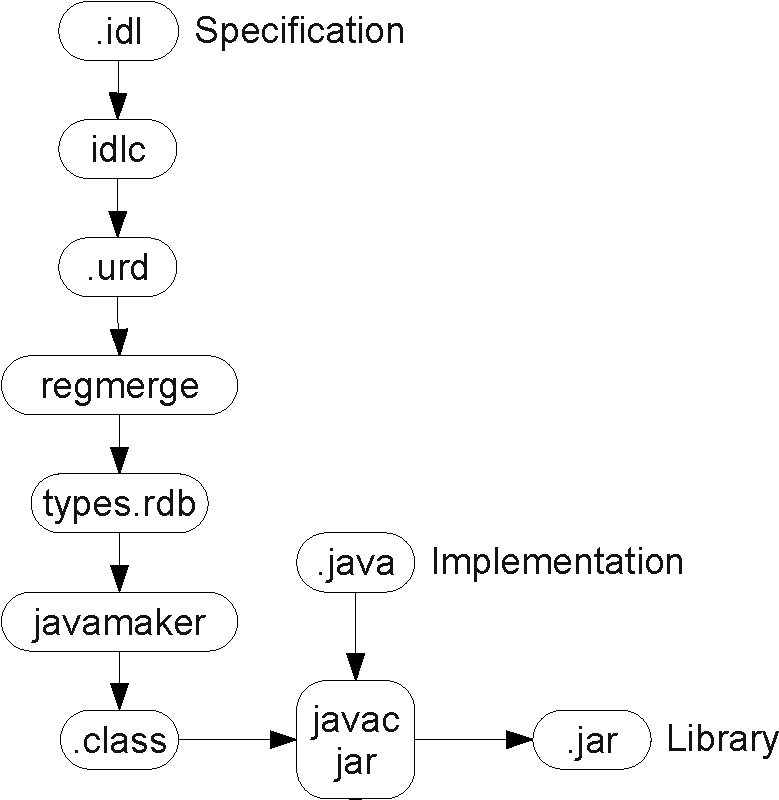
\includegraphics[width=250px,keepaspectratio]{uno-java.pdf}
\caption{Workflow of implementing an UNO service in Java}
\label{fig:uno-java}
\end{figure}

\begin{itemize}
\item \emph{idlc} compiles the .idl files to UNO Resource Descriptors,
\item \emph{regmerge} merges all the .urd files of the component to a single Resource Database,
\item \emph{javamaker} creates interfaces (.class files) from the Resource Database,
\item finally the standard Java development tools (\emph{javac}, \emph{jar})
creates the final jar, including the Java implementation.
\end{itemize}

Once the jar package is ready, a zip archive is created, containing:

\begin{itemize}
\item \emph{Addons.xcu}, containing the menu items
\item the BASIC library (callbacks for the menu items)
\item Java libraries used by the Java implementation
\item the Java implementation
\item metamodel of the stored settings
\item other files: metadata, extension description, license, etc.
\end{itemize}

\section{Workflows}

\subsection{Application servers}

The term application server is used to describe the software framework on which
the business logic of an application runs. The application server typically
interacts with SQL database servers, file server or web servers.

\subsubsection*{Web application servers}

A common usage of application servers is a web application server, where the
framework handles common web-related tasks, so that application developers can
focus on the development of the software project itself. Such common tasks
include, but not limited to:

\begin{itemize}
\item handling connections towards the database layer
\item handling incoming requests from the HTTP server
\item management of a cluster
\item load-balancing features
\item fail-over capabilities
\item centralized configuration
\item security: cryptographic and authentication features
\end{itemize}

Given that the integration between a contained application and server framework
is strong, it is a common practice to use the same programming language to
implement both. As a consequence, e.g. Java applications usually run on
application servers implemented in Java, and so on.

There are two approaches\footnote{A third, but not ineffective method is to
execute the interpreter of the programming language each time a request is
served, referred as Common Gateway Interface (CGI).} to match this requirement.
One approach is to use a generic web server, for example the Apache HTTP
Server \cite{apache-httpd}. Given that almost all programming languages has a C
API to interact with managed code, plugins for the web server can be
implemented in C to execute managed code when a HTTP requests arrives,
addressing the application in question.

The other approach is to have a dedicated HTTP server, which can only execute
applications written in a given programming language, but it so more
effectively. Supported programming languages include:

\begin{itemize}
\item .NET: both Microsoft and 3rd-party application servers are available.
Microsoft provides this functionality in their Windows Server product and their
.NET Framework.
\item Java: we will discuss this in detail below.
\item PHP: Zend Technologies produces Zend Server to host PHP applications.
\item Ruby: the Ruby on Rails framework includes the WEBrick HTTP server.
\end{itemize}

Note that though those are less popular, application servers providing support
to execute BASIC, C++, Lisp, Haskell, Python, Perl, Smalltalk or Tcl code are
also available.

\subsubsection*{Java application servers}

Java application servers have the benefit of implementing common interfaces:
that way changing application servers is supposed to be an easy operation.

These common interfaces live under the \emph{javax.servlet} namespace \cite{javax-servlet}.
Some of the included concepts:

\begin{itemize}
\item The \emph{Servlet} interface: an implementing class runs within a web
server. Its most used implementation is the \emph{HttpServlet} class, that can
handle HTTP GET, PUT, POST and DELETE requests.
\item The application can be packaged to a \emph{WAR} file before it is deployed
on the application server.
\item Servlets are invoked by a \emph{web container}, the module of the
application server directly interacting with servlets.
\item Template-based output can be generated using \emph{JavaServer Pages}
(JSP). Such templates are processed by the JavaServer Pages compiler.
\end{itemize}

Popular Java application server implementations include:

\begin{itemize}
\item GlassFish: An open-source Java application server, started by Sun
Microsystems for the Java EE platform, and it is still supported by Oracle. The
name of the product with commercial support is Oracle GlassFish Server.
\item JBoss Application Server: a detailed discussion is below.
\item Apache Tomcat: This is the application server implemented by the Apache
Software foundation, providing an implementation of the Java Servlet and
JavaServer Pages specifications.
\item IBM WebSphere Application Server (WAS): A commercial Java application
server from IBM.
\end{itemize}

\subsubsection*{JBoss}

JBoss Application server (in short, JBoss AS) is an open-source application server
based on Java EE, originally developed by JBoss, Inc -- now a division of Red
Hat. Besides implementing a server on top of Java, it even implements the Java
EE specification as well.  JBoss is written in pure Java, meaning that it is
usable on any operating system Java runs on.

At the time of writing, the latest stable version of JBoss is AS7, which
introduces a rewritten code, focusing on parallel execution, radically speeding
up start-up time \cite{jboss-fast}.

However, AS 7 is quite new, it was released on July 12, 2011 -- what we used as
a workflow engine is AS 5.1, as that was the best supported by other components
we executed inside JBoss.

JBoss provides the common application server features, including:

\begin{itemize}
\item clustering and load-balancing
\item fail-over, even if sessions are configured
\item an implementation of the Authentication and Authorization Service (JAAS)
specification
\item management and monitoring though Java Management Extensions (JMX)
\item implementation of Java Persistence API (JPA), though Hibernate
\item implementation of JavaServer Pages and / Java Servlet, through Tomcat
\item integrated support for Java Database Connectivity (JDBC)
\item OSGi support, which means one can deploy OSGi bundles in a JBoss server,
next to other existing non-OSGi deployments
\end{itemize}

JBoss itself is open-source, though commercial support is available from Red Hat.

\subsection{Workflow engines}

\subsubsection*{What is a workflow engine}

As already mentioned in the \emph{Introduction} chapter, a workflow engine
manages process definitions and instances. The primary functionality the engine
itself provides is the ability to execute these instances, storing the state of
the process instance in a permanent database. Once the process is finished, it
becomes a \emph{historic} process instance, which is still stored.

A process definition consists of nodes, which can be executed:

\begin{itemize}
\item manually: human tasks are for this purpose
\item automatically: script tasks, diverging or converging gateways are in this category
\end{itemize}

Additionally, each node can have several properties, for example imperative code
attached to a script task or due date for a human task.

The architecture of a workflow engine is event-based, changes to process
instances are triggered by events:

\begin{itemize}
\item internal events: when a deadline is reached
\item external events: when a task is completed, a trigger in an other
application starts a new process instance, etc.
\end{itemize}

When executing actions for external events, the following steps are implemented:

\begin{itemize}
\item Check if the requested action is valid in the active state (i.e. there is a transition from the current state to the requested state in the process definition).
\item Authorize the caller to determine if executing the action is permitted by the user.
\item Executing the action itself: once the operation finished, act based on its exit code (initiate error handling if necessary).
\end{itemize}

There are two popular standards to describe a process definition:

\begin{itemize}
\item Business Process Execution Language (BPEL): is standard describing an
executable language where the business process interacts with web services.
\item Business Process Model and Notation (BPMN): we will discuss it in the
next subsection in detail.
\item jBPM Process Definition Language (JPDL): a proprietary language developed
by JBoss, focusing on readability.
\end{itemize}

\subsubsection*{Operation modes}

A workflow engine can have two different operation modes. The first follows a
client-server model. \autoref{fig:workflow-server} shows this situation,
where the workflow engine is behind a server interface.

\begin{figure}[H]
\centering
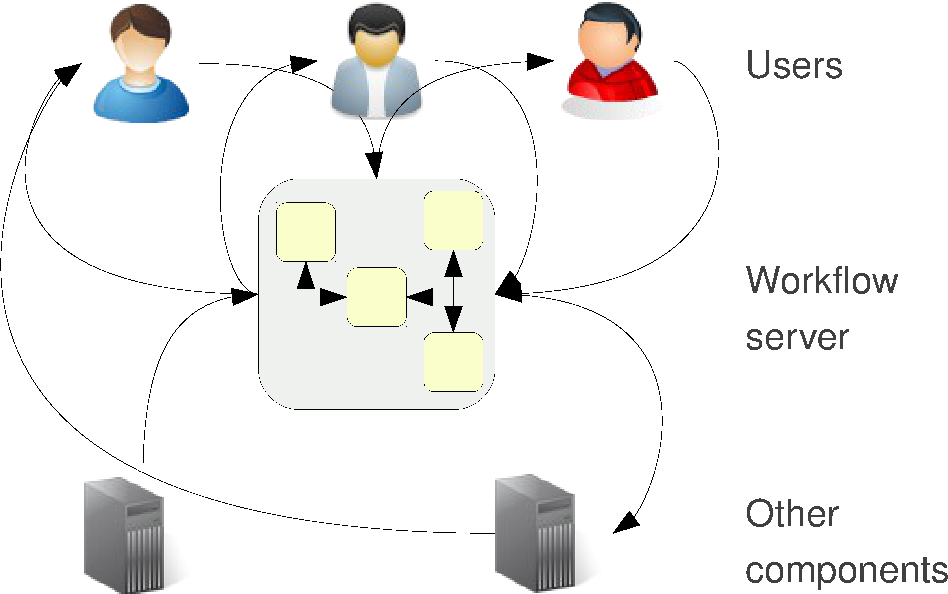
\includegraphics[width=300px,keepaspectratio]{workflow-server.pdf}
\caption{A workflow engine in server mode}
\label{fig:workflow-server}
\end{figure}

For example, in case of jBPM there is a REST API available for clients to
interact with the engine. The benefit is that the workflow server can run on a
separate machine, also no need to start or stop it when clients start or stop.
Additionally, multiple clients can connect to the workflow server at the same
time.

\autoref{fig:workflow-embedded} describes the second, embedded mode.

\begin{figure}[H]
\centering
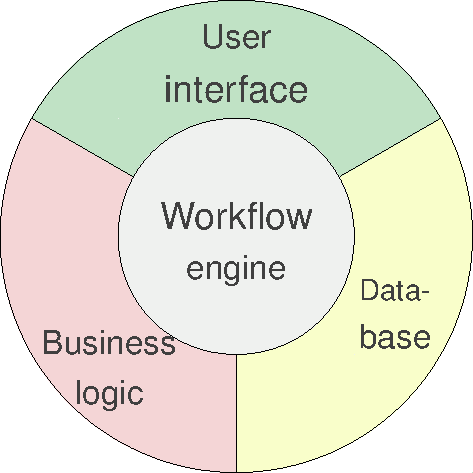
\includegraphics[width=200px,keepaspectratio]{workflow-embedded.pdf}
\caption{A workflow engine in embedded mode}
\label{fig:workflow-embedded}
\end{figure}

In this case the application and the workflow server can run in the same
process, the workflow engine is used as a simple library, which produces
increased performance.

\subsubsection*{jBPM}

jBPM \cite{jbpm} is an open-source business process manager, implemented in
Java. One property that makes it different from other workflow engines is that
it tries to give better support for developers as well. Usually workflow
engines target non-technical people, making the life of users already used to
imperative programming hard.

The biggest jBPM contributor is Red Hat, as a consequence it is not surprising
that -- when using it as a server -- the project runs best on the JBoss
application server.

The core supports executing processes defined according to the BPMN 2.0
specification\footnote{Previously it only supported the jPDL language.}. On top of that, it offers more:

\begin{itemize}
\item a web-based and an Eclipse plugin to design process definitions using an easy drag and drop method
\item its storage back-end can be any database which is supported by JPA
\item handling of human tasks is a separate component -- a sample implementation is included in the release
\item a BPM console (detailed later in the last section of this chapter), built
on top of the core provides web-based management and monitoring interface for
process instances and tasks
\item a repository, named Guvnor, can be optionally used to deploy processes to
\item the storage backend can log all detailed needed for audit functionality
\end{itemize}

Script tasks can be implemented in multiple imperative languages:

\begin{itemize}
\item MVFLEX Expression Language (MVEL): a hybrid dynamically/statically typed scripting language
\item Java
\end{itemize}

Given the above features, jBPM is an excellent candidate to serve as a workflow
server for our LibreOffice extension.

\subsection{Business Process Model and Notation}

\subsubsection*{What is business process modelling?}

Business process modelling is a process of three steps:

\begin{itemize}
\item find nodes: have a look at the real-world process and split it to a sequence of individual steps
\item node properties: define additional properties for nodes, such as the description or due date
\item transition between nodes: once transitions are declared, we can have an executable process definition
\end{itemize}

The Business Process Model and Notation (BPMN) standard \cite{bpmn} supports all
these steps, \autoref{fig:bpmn-sample} shows such a completely defined
process definition, using the Eclipse tool of jBPM.

\begin{figure}[H]
\centering
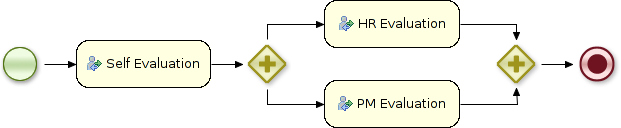
\includegraphics[width=250px,keepaspectratio]{bpmn-sample.png}
\caption{A simple BPMN process with three human tasks and two gateways}
\label{fig:bpmn-sample}
\end{figure}

The rest of this subsection gives a brief introduction to BPMN concepts used in
the later chapters of this thesis. Due to size limitations, we didn't consider
describing all types of each concept here.

\subsubsection*{BPMN basic concepts}

The most important elements in a process definition are nodes, and transitions
between these nodes. \autoref{fig:bpmn-diagram-elements} shows that BPMN
uses the following concepts to represent these:

\begin{itemize}
\item activities: a step of the real-word process: for example a human task or a script task
\item events: represent the start and end of a process, crossing a deadline or error handling
\item gateways: diverging and converging gateways model parallelism and choices
\item connectors: declare valid transitions between elements
\end{itemize}

\begin{figure}[H]
\centering
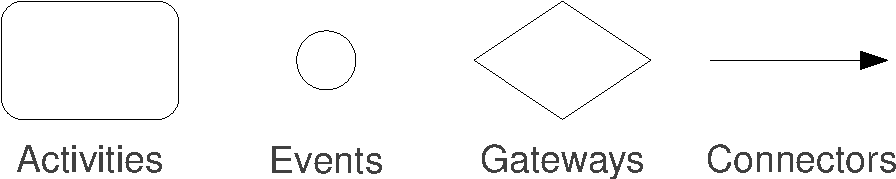
\includegraphics[width=250px,keepaspectratio]{bpmn-diagram-elements.pdf}
\caption{The basic diagram elements of BPMN}
\label{fig:bpmn-diagram-elements}
\end{figure}

\autoref{fig:bpmn-activity-types} shows there are two types of activities: tasks and subprocesses.

\begin{itemize}
\item tasks are part of a process definition that are not described in more detail
\item subprocesses refer to reusable independent parts of process definition
\end{itemize}

\begin{figure}[H]
\centering
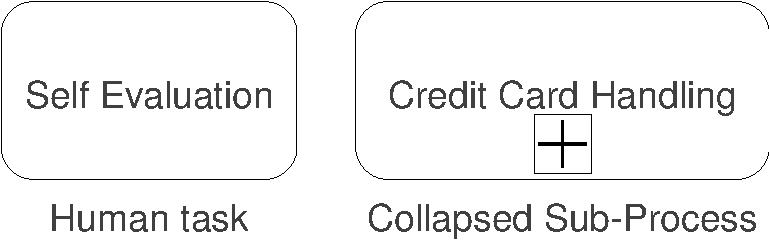
\includegraphics[width=250px,keepaspectratio]{bpmn-activity-types.pdf}
\caption{Activity types in BPMN}
\label{fig:bpmn-activity-types}
\end{figure}

BPMN supports start, intermediate and stop events. Start events mark where the
execution of the process will begin. \autoref{fig:bpmn-start-event-types}
shows three start even types:

\begin{itemize}
\item normal start is used when an explicit start invoked the process
\item message start indicates the process was triggered by receiving a message
\item rule start means the process was activated by a business rule
\end{itemize}

\begin{figure}[H]
\centering

\includegraphics[width=200px,keepaspectratio]{bpmn-start-event-types.pdf}
\caption{Three start event types in BPMN}
\label{fig:bpmn-start-event-types}
\end{figure}

Intermediate events can occur anytime after the start, but before the end. They
can be (see \autoref{fig:bpmn-intermediate-event-types}):

\begin{itemize}
\item normal events are generated by activities
\item timer events can occur when crossing deadlines
\item compensation events can occur when rolling back a transaction
\end{itemize}

\begin{figure}[H]
\centering

\includegraphics[width=200px,keepaspectratio]{bpmn-intermediate-event-types.pdf}
\caption{Three intermediate event types in BPMN}
\label{fig:bpmn-intermediate-event-types}
\end{figure}

Finally end events indicate that the main process ended. Subtypes shown on
\autoref{fig:bpmn-end-event-types}:

\begin{itemize}
\item none end means the main process ended, but subprocesses are still running
\item terminate end indicates the execution of the process instance ends
\item error end describes something unexpected happened
\end{itemize}

\begin{figure}[H]
\centering

\includegraphics[width=200px,keepaspectratio]{bpmn-end-event-types.pdf}
\caption{Three end event types in BPMN}
\label{fig:bpmn-end-event-types}
\end{figure}

The two most common used gateway types (\autoref{fig:bpmn-gateway-types}):

\begin{itemize}
\item exclusive gateway (can also be marked with an internal ``X''): only one branch is executed
\item parallel gateway: branches are executed in parallel
\end{itemize}

\begin{figure}[H]
\centering

\includegraphics[width=150px,keepaspectratio]{bpmn-gateway-types.pdf}
\caption{Two gateway types in BPMN}
\label{fig:bpmn-gateway-types}
\end{figure}

The last BPMN type we introduce here are connectors. Three type of them can be
seen on \autoref{fig:bpmn-connector-types}:

\begin{itemize}
\item sequence flow is used for ordering between tasks
\item message flow indicates two activities are prepared to send / receive messages
\item association is used to assign additional data to activities
\end{itemize}

\begin{figure}[H]
\centering
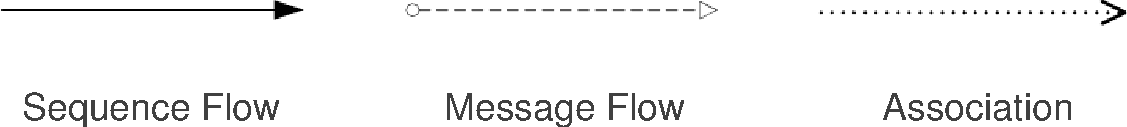
\includegraphics[width=300px,keepaspectratio]{bpmn-connector-types.pdf}
\caption{Three connector types in BPMN}
\label{fig:bpmn-connector-types}
\end{figure}

\subsubsection*{BPMN support in jBPM}

jBPM 3.x and earlier supported the jPDL format declare process definitions.
jBPM 4.x introduced support for BPMN, while jBPM 5.x supports BPMN exclusively.
Tools are available to somewhat automate the conversion from jPDL to BPMN.

\subsection{Object-Relational Mapping}

Both jBPM itself and its sample human task server implementation uses
object-relational mapping (ORM) to store data in SQL. The general problem is
that object-oriented applications store runtime data in object, while
persistent data store can't store object as-is, code has to be written manually
to store and restore object to / from a relational database.

An ORM automates this procedure, reducing code needed to be implemented
manually. A disadvantage of using an ORM can be that highly optimised
hand-constructed queries are faster then the ones auto-generated by the ORM. A
solution for this can be the usage of stored procedures, in case portability
between storage back-ends is not a requirement.

In case of Java, the de facto ORM tool is hibernate, jBPM uses that as well.
Hibernate introduces the Hibernate Query Language (HQL), which is fully-object
oriented: on one hand that means it understands inheritance and polymorphism,
on the other hand it still provides flexibility similar to the traditional
stored procedures.

\subsection{The BPM Console}

\subsubsection*{Technical overview}

\begin{figure}[H]
\centering
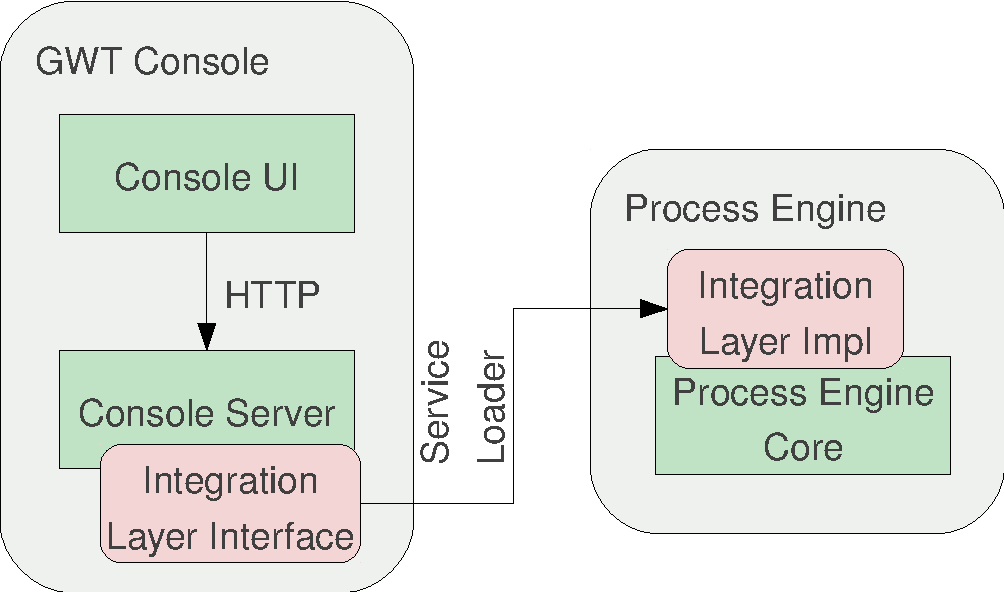
\includegraphics[width=300px,keepaspectratio]{bpm-console.pdf}
\caption{Components of the BPM console}
\label{fig:bpm-console}
\end{figure}

The BPM Console is a generic web console for process engines. In practice it is
used by:

\begin{itemize}
\item Riftsaw: a BPEL engine
\item jBPM: a BPMN engine
\item Drools: a business logic integration platform
\end{itemize}

Components are shown on \autoref{fig:bpm-console}:

\begin{itemize}
\item the integration layer is an interface to be implemented by process engines
\item the console server provides a REST API and translates HTTP requests to the integration layer
\item the web console is a Google Web Toolkit (GWT) application communicating with the console server only
\end{itemize}

The integration layer discovers the available implementation using the standard
J2EE service loader mechanism \cite{service-loader}. The console-related
articats are described in \autoref{tab:bpm-components}.

\begin{table}[H]
  \begin{center}
    \begin{tabular}{| l | l |}
    \hline
    \textbf{Archive name} & \textbf{Description} \\ \hline
    gwt-console.war & The user interface \\ \hline
    gwt-console-server.war & The REST server \\ \hline
    gwt-console-rpc.jar & Domain model \\ \hline
    gwt-console-server-integration.jar & Integration layer \\ \hline
    \end{tabular}
  \end{center}
  \caption{Artifacts of the BPM console}
  \label{tab:bpm-components}
\end{table}

\subsubsection*{Workspace framework}

The workspace of the BPM console is a concept completely independent from the
document server workspace. The workspace here is the user interface of the web
console. The workspace features editors. These editors are implementing a
common API, and they serve two purposes:

\begin{itemize}
\item they can be used for management of the workflow engine
\item they serve as an example on how to use the console server
\end{itemize}

The editor interface implementations are called \emph{buildtime plugins}. For our
purposes, two plugins are interesting:

\begin{itemize}
\item \emph{ProcessEditor}: can be used to edit process instances: start, inspect or terminate
\item \emph{TaskEditor}: can be used to complete, claim, release tasks
\end{itemize}

Both of these editors are specific to jBPM, the list of loaded plugins is
determined build-time: a \emph{profile} can be specified as a parameter of the
build process, and the jBPM profile lists these plugins. As a result, the
selected profile becomes the \emph{workspace configuration}.

The console server supports \emph{runtime plugins}. These are:

\begin{itemize}
\item FormDispatcherPlugin: handles the completion of task forms
\item GraphViewerPlugin: handles rendering of the current state of a process instance
\item ProcessEnginePlugin: handles management of the process definitions
\end{itemize}

The same service loader mechanism is used to load the implementation of these
interfaces as for the integration layer, however in case these are not
available, then the related functionality is simply hidden from the web
interface, it does not cause a fatal error.

\subsubsection*{Management capabilities}

Management capabilities are determined by the installed editor plugins. The
project suggests that they try to keep a balance between:

\begin{itemize}
\item providing plugins which are examples only
\item supporting every corner case
\end{itemize}

The process editor offers the following features:

\begin{itemize}
\item Management of the life cycle of process instances: process instances can
be started, terminated or deleted. Termination ends the process instance,
deletion also removes the history information.
\item Visualization of process activity: the already mentioned
\emph{GraphViewerPlugin} can draw the graphical representation of the BPMN
definition and show the actual instance state.
\item Instance data can be inspected: variables associated with a given process
instance can be accessed read-only.
\item Process form handling: if the process definition has a form associated
(which is the way to start parametrized workflows), it will show it and let
the user fill it out before the process instance starts.
\end{itemize}

The task editor can manage tasks of the currently logged in user. It features:

\begin{itemize}
\item a personal and a group task lister
\item a manager for the task life cycle: it can be open or assigned (whenever it is completed, it gets removed from the list, so there is no such state in the user interface)
\item a handler for task forms: whenever the task has an associated form, the user can provide input or review read-only data
\end{itemize}
